% Options for packages loaded elsewhere
\PassOptionsToPackage{unicode}{hyperref}
\PassOptionsToPackage{hyphens}{url}
\PassOptionsToPackage{dvipsnames,svgnames,x11names}{xcolor}
%
\documentclass[
  11pt,
  ignorenonframetext,
  fontset=fandol]{beamer}
\usepackage{pgfpages}
\setbeamertemplate{caption}[numbered]
\setbeamertemplate{caption label separator}{: }
\setbeamercolor{caption name}{fg=normal text.fg}
\beamertemplatenavigationsymbolsempty
% Prevent slide breaks in the middle of a paragraph
\widowpenalties 1 10000
\raggedbottom
\setbeamertemplate{part page}{
  \centering
  \begin{beamercolorbox}[sep=16pt,center]{part title}
    \usebeamerfont{part title}\insertpart\par
  \end{beamercolorbox}
}
\setbeamertemplate{section page}{
  \centering
  \begin{beamercolorbox}[sep=12pt,center]{part title}
    \usebeamerfont{section title}\insertsection\par
  \end{beamercolorbox}
}
\setbeamertemplate{subsection page}{
  \centering
  \begin{beamercolorbox}[sep=8pt,center]{part title}
    \usebeamerfont{subsection title}\insertsubsection\par
  \end{beamercolorbox}
}
\AtBeginPart{
  \frame{\partpage}
}
\AtBeginSection{
  \ifbibliography
  \else
    \frame{\sectionpage}
  \fi
}
\AtBeginSubsection{
  \frame{\subsectionpage}
}
\usepackage{amsmath,amssymb}
\usepackage{lmodern}
\usepackage{iftex}
\ifPDFTeX
  \usepackage[T1]{fontenc}
  \usepackage[utf8]{inputenc}
  \usepackage{textcomp} % provide euro and other symbols
\else % if luatex or xetex
  \usepackage{unicode-math}
  \defaultfontfeatures{Scale=MatchLowercase}
  \defaultfontfeatures[\rmfamily]{Ligatures=TeX,Scale=1}
\fi
\usetheme[]{Singapore}
\usecolortheme{seahorse}
\usefonttheme{structurebold}
% Use upquote if available, for straight quotes in verbatim environments
\IfFileExists{upquote.sty}{\usepackage{upquote}}{}
\IfFileExists{microtype.sty}{% use microtype if available
  \usepackage[]{microtype}
  \UseMicrotypeSet[protrusion]{basicmath} % disable protrusion for tt fonts
}{}
\usepackage{xcolor}
\newif\ifbibliography
\setlength{\emergencystretch}{3em} % prevent overfull lines
\providecommand{\tightlist}{%
  \setlength{\itemsep}{0pt}\setlength{\parskip}{0pt}}
\setcounter{secnumdepth}{-\maxdimen} % remove section numbering
\logo{
\includegraphics[width=0.6in,height=0.2in]{"images/JNU1.jpg"}}
\usepackage[fontset = windows]{}
\usepackage{wrapfig}
\usepackage{tikz}
\usepackage{wallpaper}
\usepackage[default]{sourcesanspro}
\usepackage[scale=.9]{sourcecodepro}
\ifLuaTeX
  \usepackage{selnolig}  % disable illegal ligatures
\fi
\usepackage[]{natbib}
\bibliographystyle{apalike}
\IfFileExists{bookmark.sty}{\usepackage{bookmark}}{\usepackage{hyperref}}
\IfFileExists{xurl.sty}{\usepackage{xurl}}{} % add URL line breaks if available
\urlstyle{same} % disable monospaced font for URLs
\hypersetup{
  pdftitle={Interpretable Machine Learning of PET Imaging for Individualized Predictions of Seizure Outcomes after Temporal Lobe Epilepsy Surgery},
  pdfauthor={Huanhua Wu Prof.~Hao Xu\^{}\{*\} ~},
  pdfkeywords={Epilepsy, PET/CT, Radiomics, Explainable Machine
Learning},
  colorlinks=true,
  linkcolor={ForestGreen},
  filecolor={Maroon},
  citecolor={Blue},
  urlcolor={Blue},
  pdfcreator={LaTeX via pandoc}}

\title{Interpretable Machine Learning of PET Imaging for Individualized
Predictions of Seizure Outcomes after Temporal Lobe Epilepsy Surgery}
\subtitle{\emph{2022 GDMA Nuclear Medicine Annual Conference}}
\author{Huanhua Wu\\
Prof.~Hao Xu\(^{*}\) ~}
\date{2022-12-03}
\institute{The First Affiliated Hospital of Jinan University ~}

\begin{document}
\frame{\titlepage}

\begin{frame}[allowframebreaks]
  \tableofcontents[hideallsubsections]
\end{frame}
\begin{frame}
\setbeamercolor{titlelike}{bg=black,fg=white}
\newcommand\Background{%
\begin{tikzpicture}[remember picture,overlay]
\node[inner sep = 0pt, outer sep = 0pt,opacity=0.95]
  at (current page.center)
  {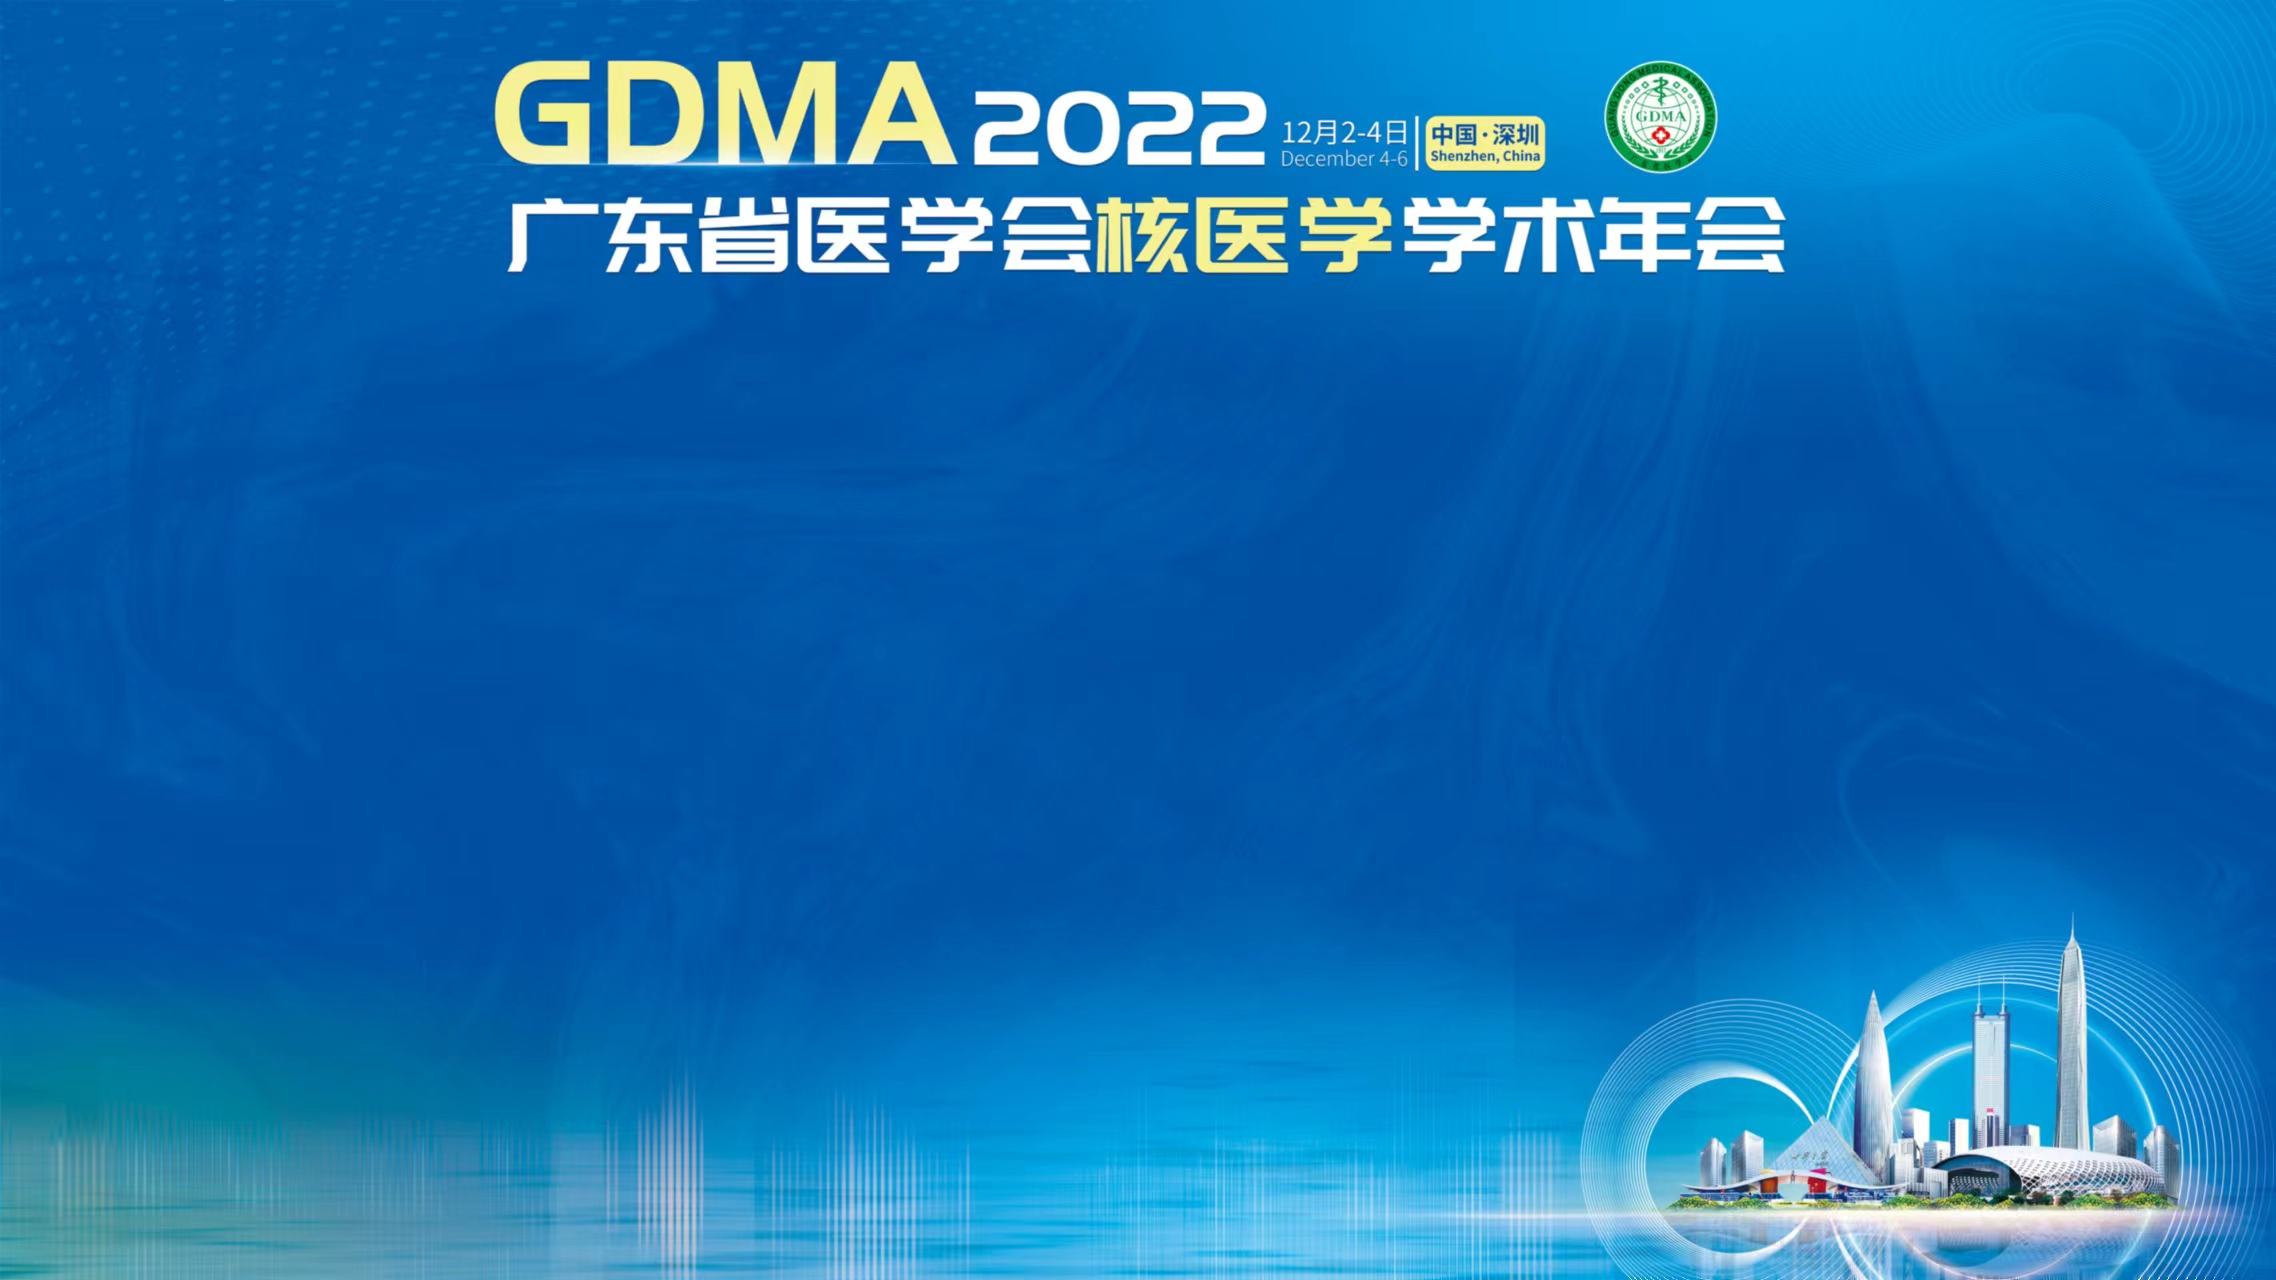
\includegraphics[width=\paperwidth,height=\paperheight]{images/GDMA.png}};
\end{tikzpicture}%
}

\def\begincols{\begin{columns}}
\def\begincol{\begin{column}}
\def\endcol{\end{column}}
\def\endcols{\end{columns}}
\end{frame}

\hypertarget{introduction}{%
\section{Introduction}\label{introduction}}

\begin{frame}{Background}
\protect\hypertarget{background}{}
\begin{figure}

{\centering 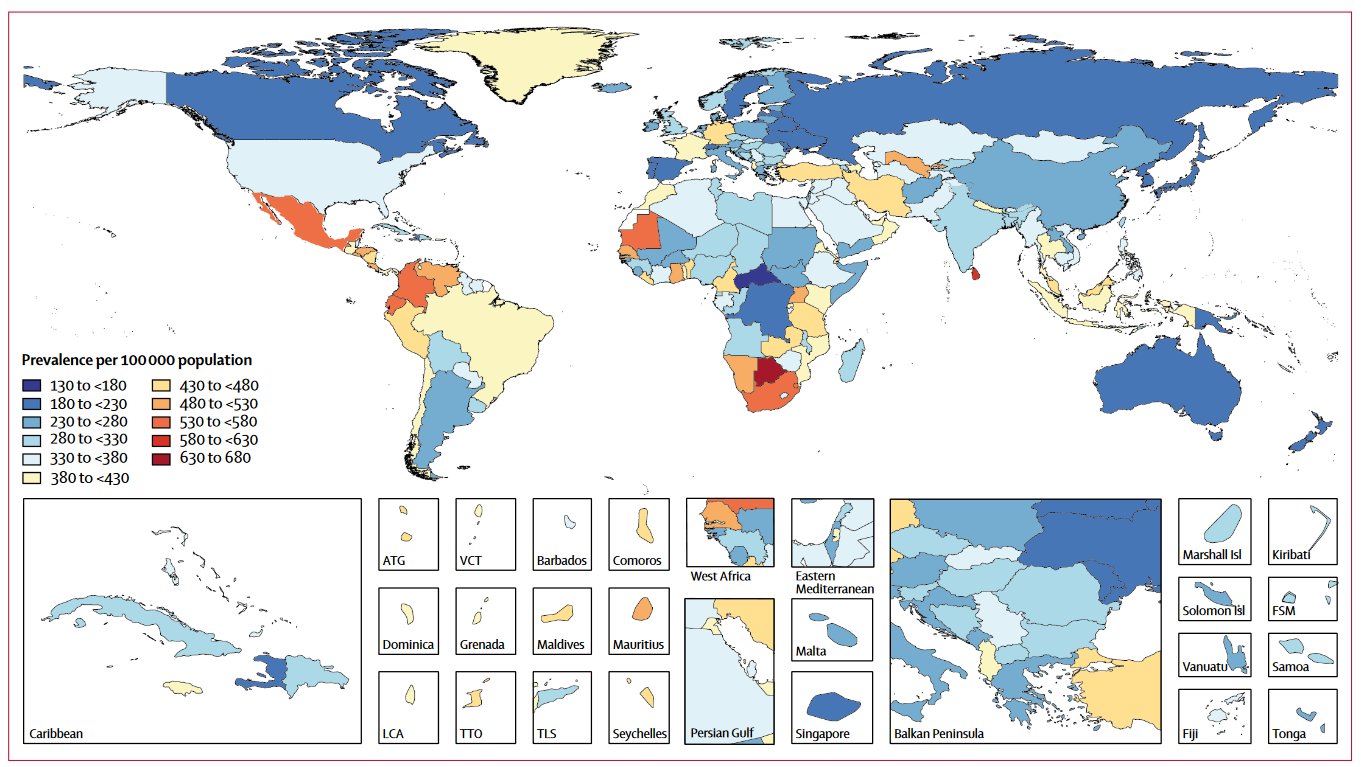
\includegraphics[width=1\linewidth]{images/global_epi} 

}

\caption{Epilepsy epidemiology}\label{fig:unnamed-chunk-2}
\end{figure}
\end{frame}

\begin{frame}{Aims}
\protect\hypertarget{aims}{}
\begin{figure}

{\centering 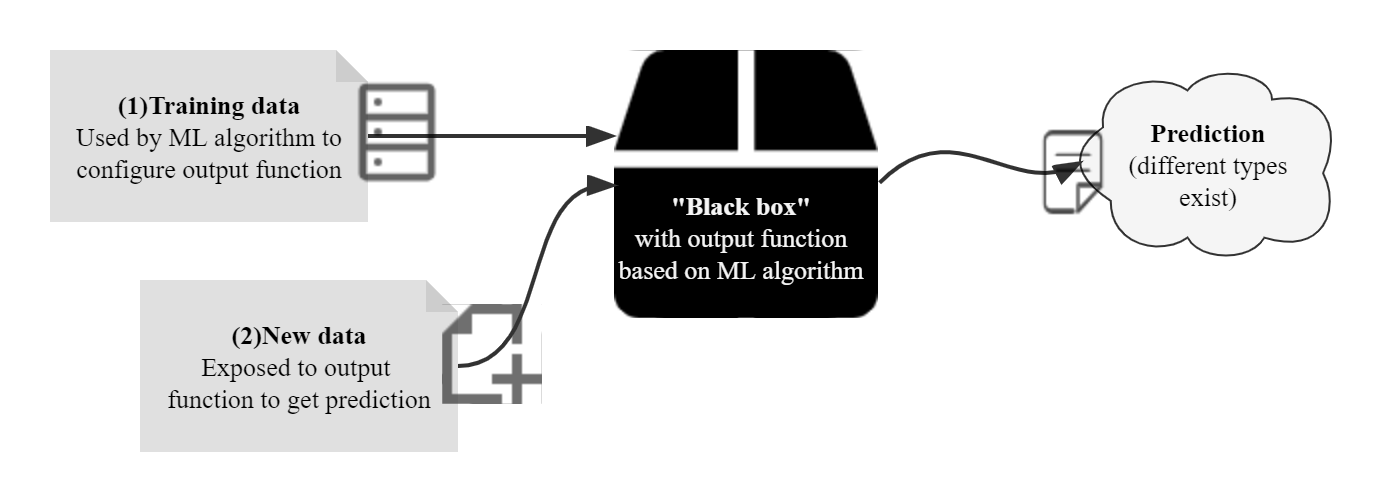
\includegraphics[width=0.7\linewidth]{images/Black-box} 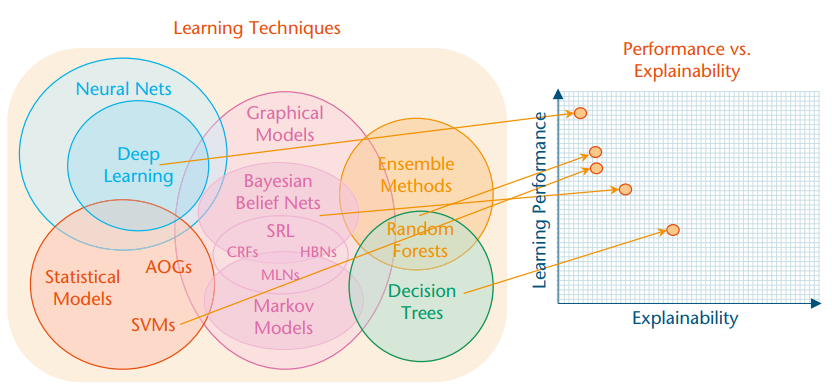
\includegraphics[width=0.8\linewidth]{images/xai} 

}

\caption{Focuses on interpretability of ML}\label{fig:unnamed-chunk-3}
\end{figure}
\end{frame}

\begin{frame}{Scheme}
\protect\hypertarget{scheme}{}
\begin{figure}

{\centering 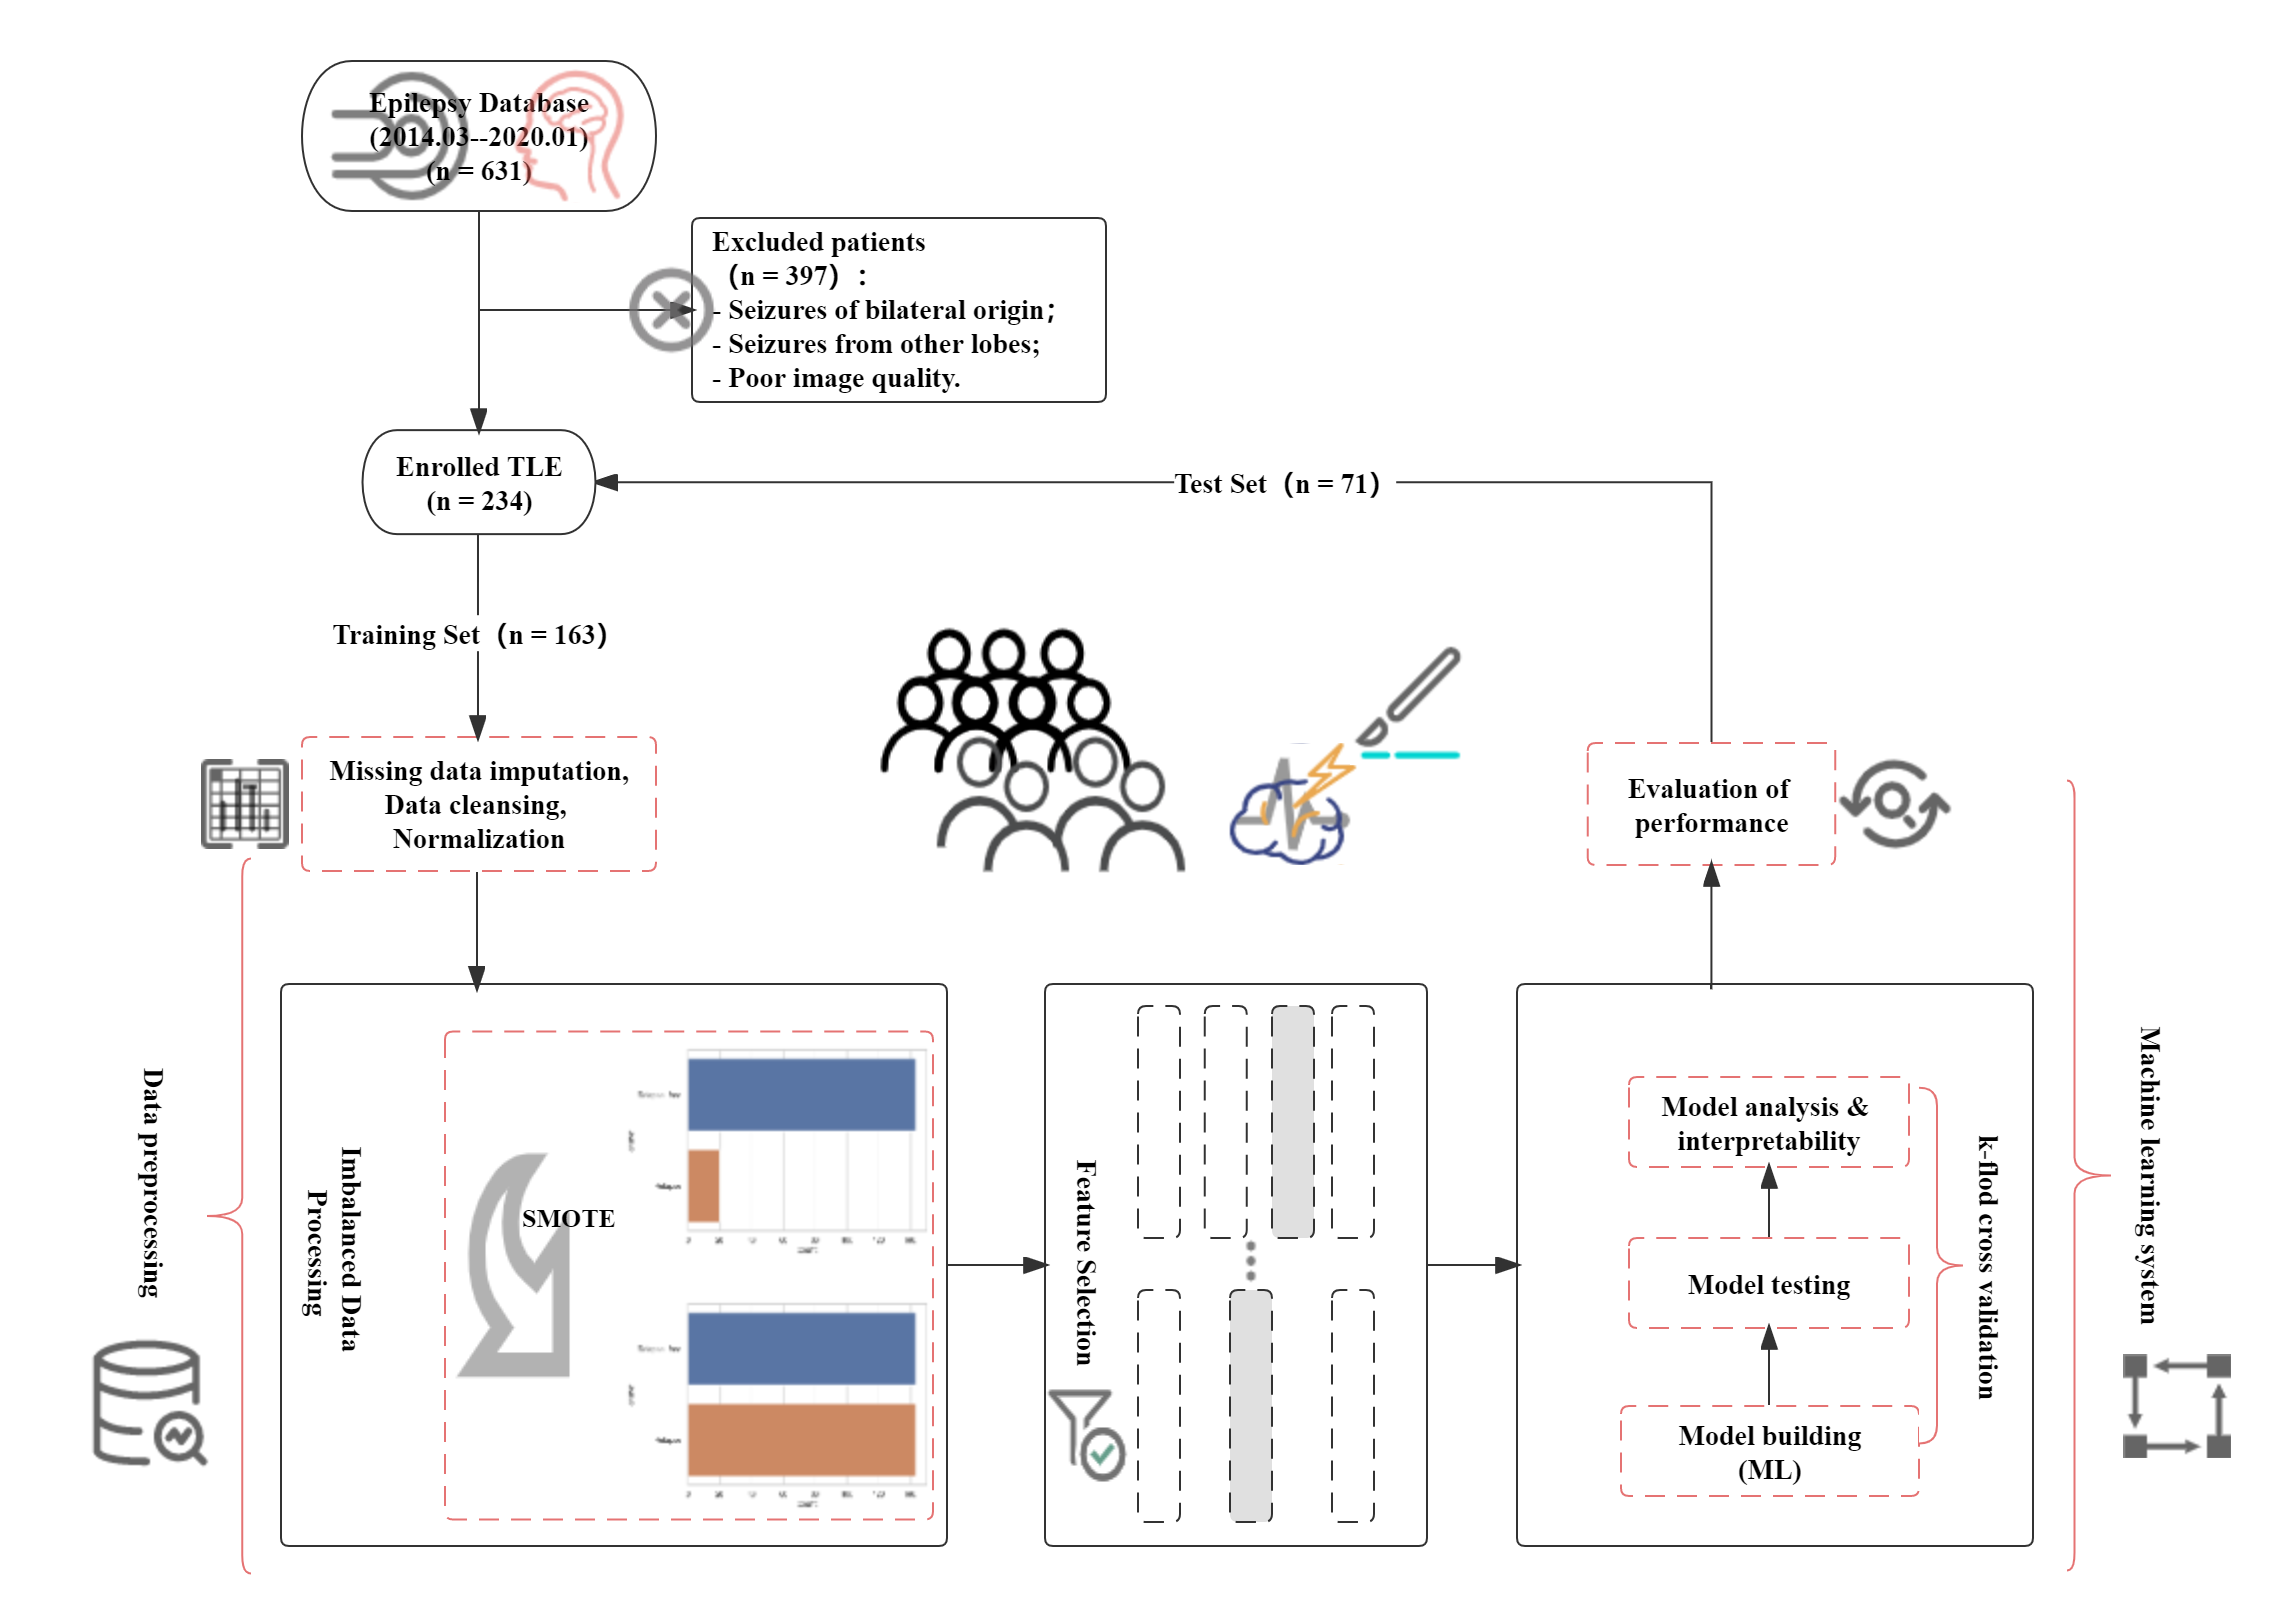
\includegraphics[width=0.85\linewidth]{images/TLE_EML_Flow} 

}

\caption{Flowchart of TLE postsurgical IML}\label{fig:unnamed-chunk-4}
\end{figure}
\end{frame}

\hypertarget{the-data}{%
\section{The Data}\label{the-data}}

\begin{frame}{Combined of PET Radiomics and Clinical Features}
\protect\hypertarget{combined-of-pet-radiomics-and-clinical-features}{}
\begin{figure}

{\centering 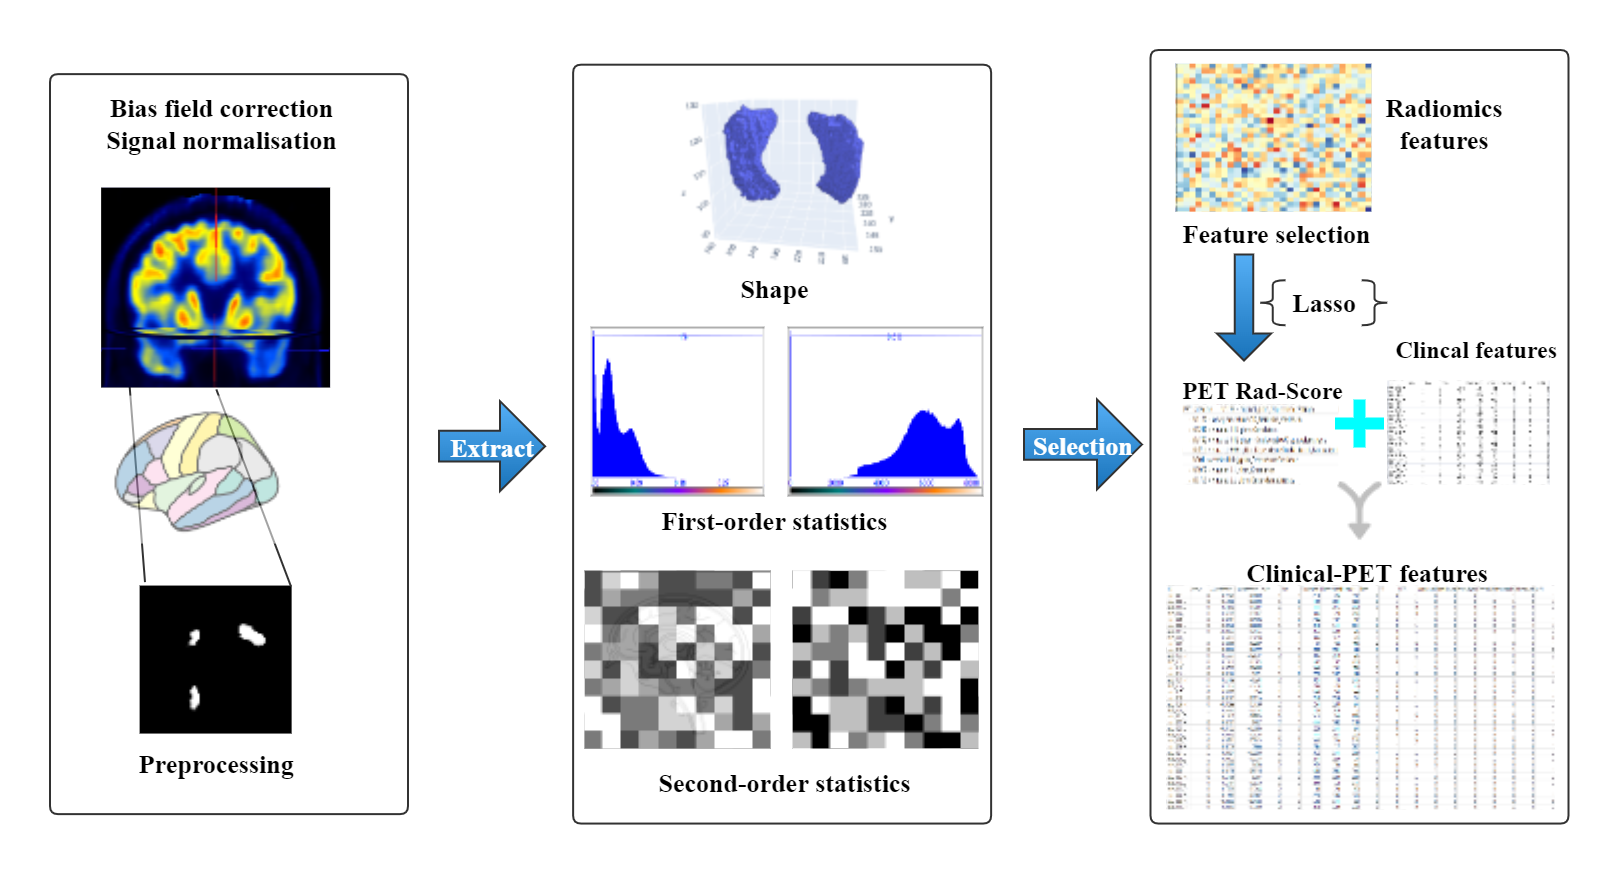
\includegraphics[width=1.1\linewidth]{images/PET_radiomics} 

}

\caption{PET radiomics  score and clinical-PET features}\label{fig:unnamed-chunk-5}
\end{figure}
\end{frame}

\begin{frame}{Exploratory Data Analysis}
\protect\hypertarget{exploratory-data-analysis}{}
\begin{figure}

{\centering \includegraphics[width=0.6\linewidth]{images/heatplot} 

}

\caption{Heatmap of Clinical-PET Features}\label{fig:unnamed-chunk-6}
\end{figure}
\end{frame}

\hypertarget{the-model}{%
\section{The Model}\label{the-model}}

\begin{frame}{Benchmark}
\protect\hypertarget{benchmark}{}
\textbf{Table 1:} Performance Comparison Eleven ML algorithms and
K-folds Cross-validation of the Selected AdaBoost

\begin{columns}
\column{.4\textwidth}
\begin{figure}
\centering
% Requires \usepackage{graphicx}
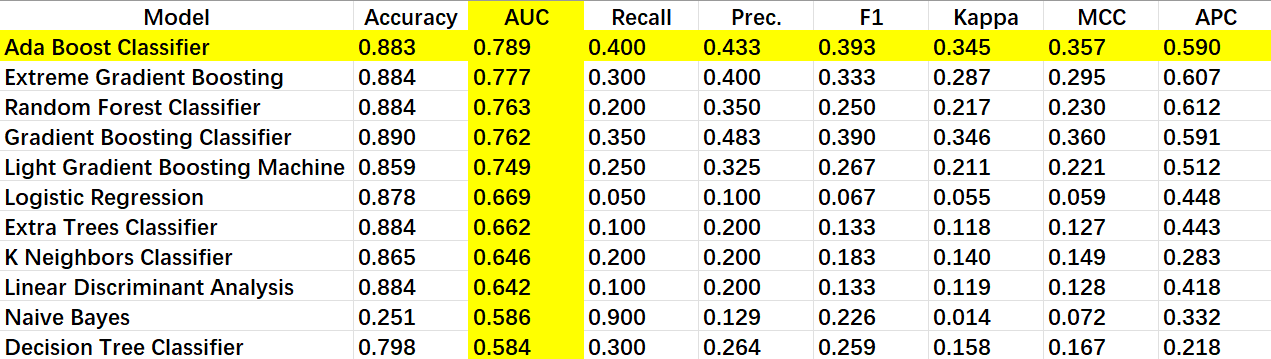
\includegraphics[width=6cm]{images/caret.png}
\end{figure}
\column{.5\textwidth}
\begin{figure}
\centering
% Requires \usepackage{graphicx}
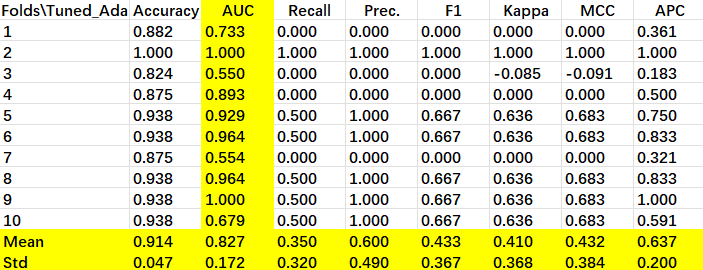
\includegraphics[width=6cm]{images/k_fold_tuned_Ada.png}
\end{figure}
\end{columns}
\end{frame}

\begin{frame}[fragile]{AdaBoost Algorithm}
\protect\hypertarget{adaboost-algorithm}{}
\begin{figure}

{\centering 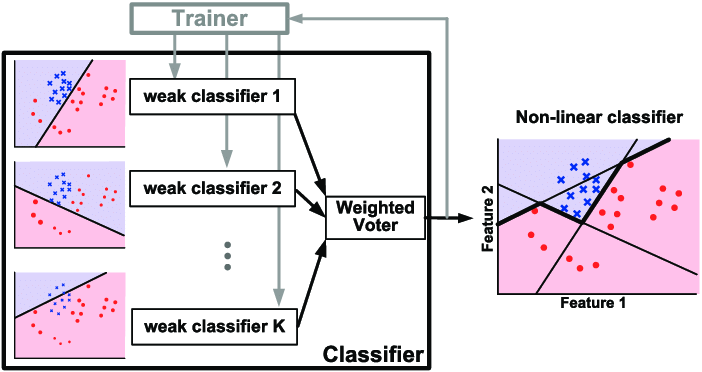
\includegraphics[width=0.8\linewidth]{images/AdaBoost} 

}

\caption{Illustration of AdaBoost Algorithm}\label{fig:unnamed-chunk-7}
\end{figure}

\begin{itemize}
\tightlist
\item
  \texttt{AdaBoostClassifier(algorithm=\textquotesingle{}SAMME\textquotesingle{},\ base\_estimator=None,\ learning\_rate=0.2,\ \ \ \ \ \ \ \ \ \ \ \ \ \ \ \ \ \ \ \ n\_estimators=230,\ random\_state=123)}
\end{itemize}
\end{frame}

\hypertarget{the-explanation}{%
\section{The Explanation}\label{the-explanation}}

\begin{frame}{Permutation Importance}
\protect\hypertarget{permutation-importance}{}
\begin{figure}

{\centering 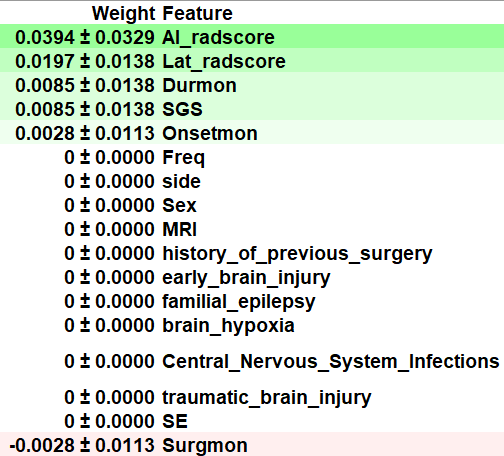
\includegraphics[width=0.6\linewidth]{images/eli5} 

}

\caption{Permutation Importance of AdaBoost}\label{fig:unnamed-chunk-8}
\end{figure}
\end{frame}

\begin{frame}{Partial Dependence Plot}
\protect\hypertarget{partial-dependence-plot}{}
\begin{figure}

{\centering 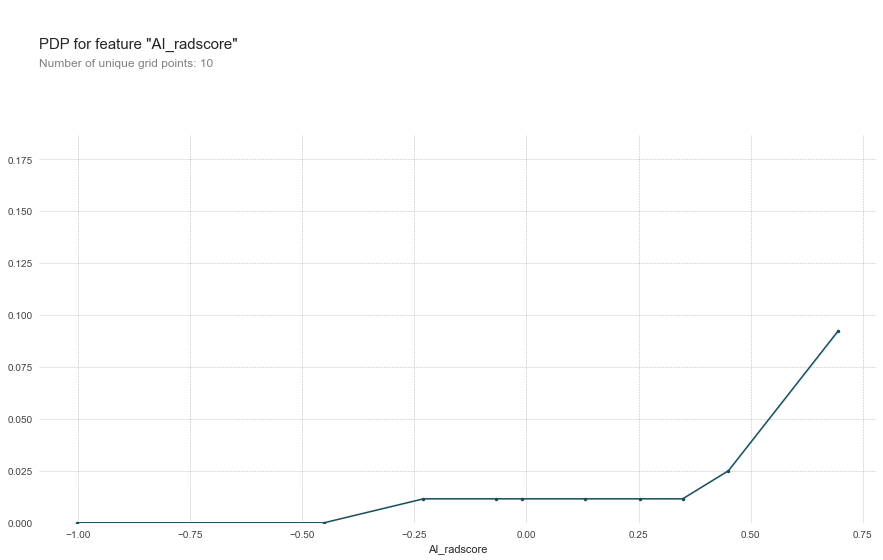
\includegraphics[width=0.8\linewidth]{images/PDP_ai} 

}

\caption{PDP plot of AI_radscore}\label{fig:unnamed-chunk-9}
\end{figure}
\end{frame}

\hypertarget{conclusion}{%
\section{Conclusion}\label{conclusion}}

\begin{frame}{Key Points}
\protect\hypertarget{key-points}{}
\begin{itemize}
\tightlist
\item
  Metabolic radiomics are helpful to predict the post-surgical seizure
  outcomes;
\item
  Combination of PET Radiomics and Clinical Features are more robust;
\item
  IML technique can further deepen the understanding of the principle of
  machine learning model and the decision-making process for
  professional and intuitive interpretation
\end{itemize}
\end{frame}

\begin{frame}{Limitations}
\protect\hypertarget{limitations}{}
\begin{itemize}
\tightlist
\item
  More data, especially external validation cohort;
\item
  Fusion of PET/MRI multimodal imaging;
\item
  Other subtypes of drug-resistant epilepsy
\end{itemize}
\end{frame}

\begin{frame}{}
\protect\hypertarget{section}{}
For more theoretical approaches to machine learning model explanation,
see
\href{https://christophm.github.io/interpretable-ml-book/}{Interpretable
Machine Learning: A Guide for Making Black Box Models Explainable},refer
to\citep{beghi2019global},\citep{rajpurkar2021deep},\citep{mlr3book},\citep{molnar2022}.

\bigskip

\textbf{Email:}
\href{mailto:wane199@outlook.com}{\nolinkurl{wane199@outlook.com}}
\end{frame}

\begin{frame}{}
\protect\hypertarget{section-1}{}
\begin{center}
  \emph{\textbf{\Huge{{THANKS !}}}}
\end{center}
%
\begin{tikzpicture}[remember picture,overlay]
\node[inner sep = 0pt, outer sep = 0pt,opacity=0.95]
  at (current page.center)
  {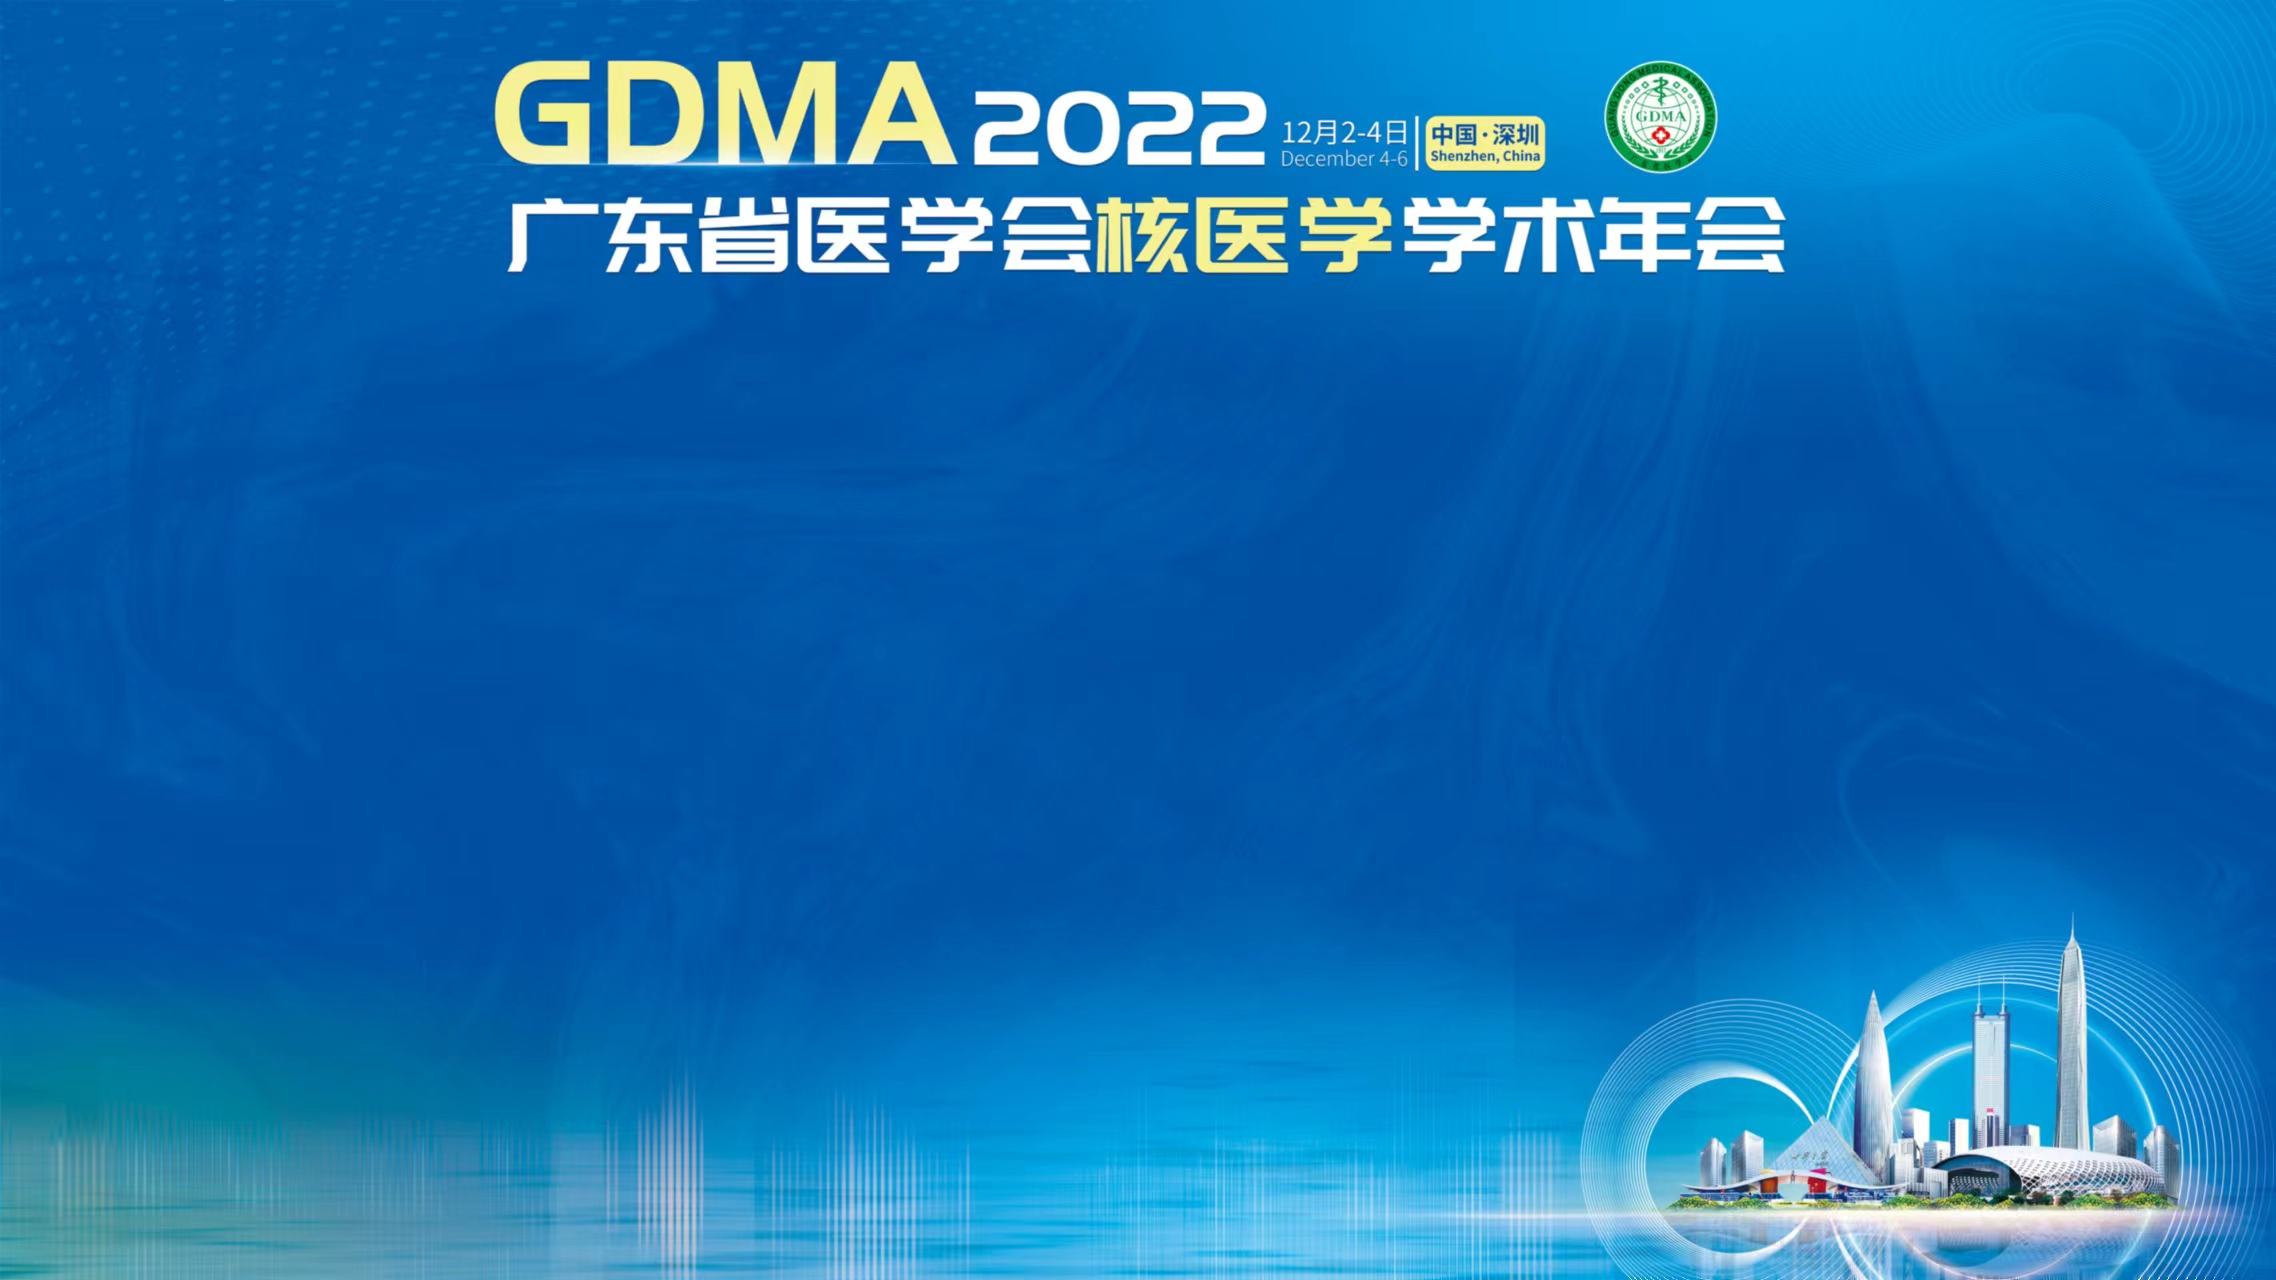
\includegraphics[width=\paperwidth,height=\paperheight]{images/GDMA.png}};
\end{tikzpicture}%
\end{frame}

\renewcommand\refname{References}
\begin{frame}[allowframebreaks]{References}
  \bibliographytrue
  \bibliography{refer.bib}
\end{frame}

\end{document}
